\section{Methods} \label{Methods}

\subsection{Subjects}

Thirty healthy subjects 
%(7 women and 23 men; mean age,%29  6 yr) 
participated in the study. The subjects were right-handed,
%(as assessed by a short questionnaire based on the Edinburgh scale),
they had normal vision or vision that was corrected to normal, and were
na\"ive to the purpose of the experiments. Two runs had to be rejected due to technical problems encountered during data acquisition. The analysis was then performed on twenty-eight subjects.

 %They gave informed consent
%to procedures approved by the Institutional Review Board of Scientific
%Institute Foundation Santa Lucia, in conformity with the Declaration
%of Helsinki on the use of human subjects in research.

\subsection{Experimental setup}

Subjects sat on a chair placed in front of a laptop screen. They were asked to 
choose a comfortable position which allowed them to see the whole screen. A blue rectangle
(the ''wall'', 6.24 cm large and long as the height of the screen) was constantly displayed 
0.26 cm from the right side of the screen against a black background. In each trial a red square (the ''ball'', 
0.13 cm side) flew following a parabolic trajectory from the left to the right side of the screen at predefined initial 
vertical position, initial velocity and acceleration (see Protocols). It neither disappeared over or under the screen boundaries nor bounced, but it became invisible when it passed behind the wall. Ball trajectories were generated from the simple equation:
\begin{eqnarray} \label{Eq:Trajectories}
\underline{x}(t) = \underline{x}_0 + \underline{v}_0 \cdot t +  \frac{1}{2} \cdot \underline{a} \cdot t^2
\end{eqnarray}
where:
\begin{itemize}
	\item $\underline{x} = \left[x, y\right]$ ball coordinates on the screen at time t,
	\item $\underline{x}_0 = \left[x_0, y_0\right]$ initial ball position,
	\item $\underline{v}_0 = \left[v_{x0}, v_{y0}\right]$ initial ball velocity,
	\item  $\underline{a} = \left[a_x, a_y\right]$ constant ball acceleration.
\end{itemize}

Practically, Eq. (\ref{Eq:Trajectories}) simulates a two dimensional ballistic flight of the ball
subject to a constant acceleration $\underline{a}$. The initial position ($\underline{x}_0$) and velocity ($\underline{v}_0$) were changed from to trial to trial so as to have a different (though always parabolic) trajectory.

At the extreme right of the scene a light blue rectangle was located (the ``paddle'', 0.26 cm large and 0.52 cm long), which could be moved along the vertical direction by the subject. This was achieved by recording the position of subject's right hand along the vertical axis and converting it into the vertical position of the paddle, in the video game reference frame. 
Positions were measured through a magnetic tracker (Flock of Birds, Ascension Technology, Burlington, VT) whose sensor was clasped by subjects in their right hand. Each downward or upward hand displacement corresponded to an equivalent paddle displacement on the screen. During a calibration phase performed before the beginning of the experiment, subjects were asked to choose their starting hand position so as to have the possibility to move comfortably about 10 cm upwards and 10 cm downwards. The corresponding paddle position was fixed at the center of the screen height. In this way subjects could easily reach the screen boundaries.
See Fig.\ref{figSchemaPong} for a sketch of the screen.

\begin{figure}[tbp]
	\centering
		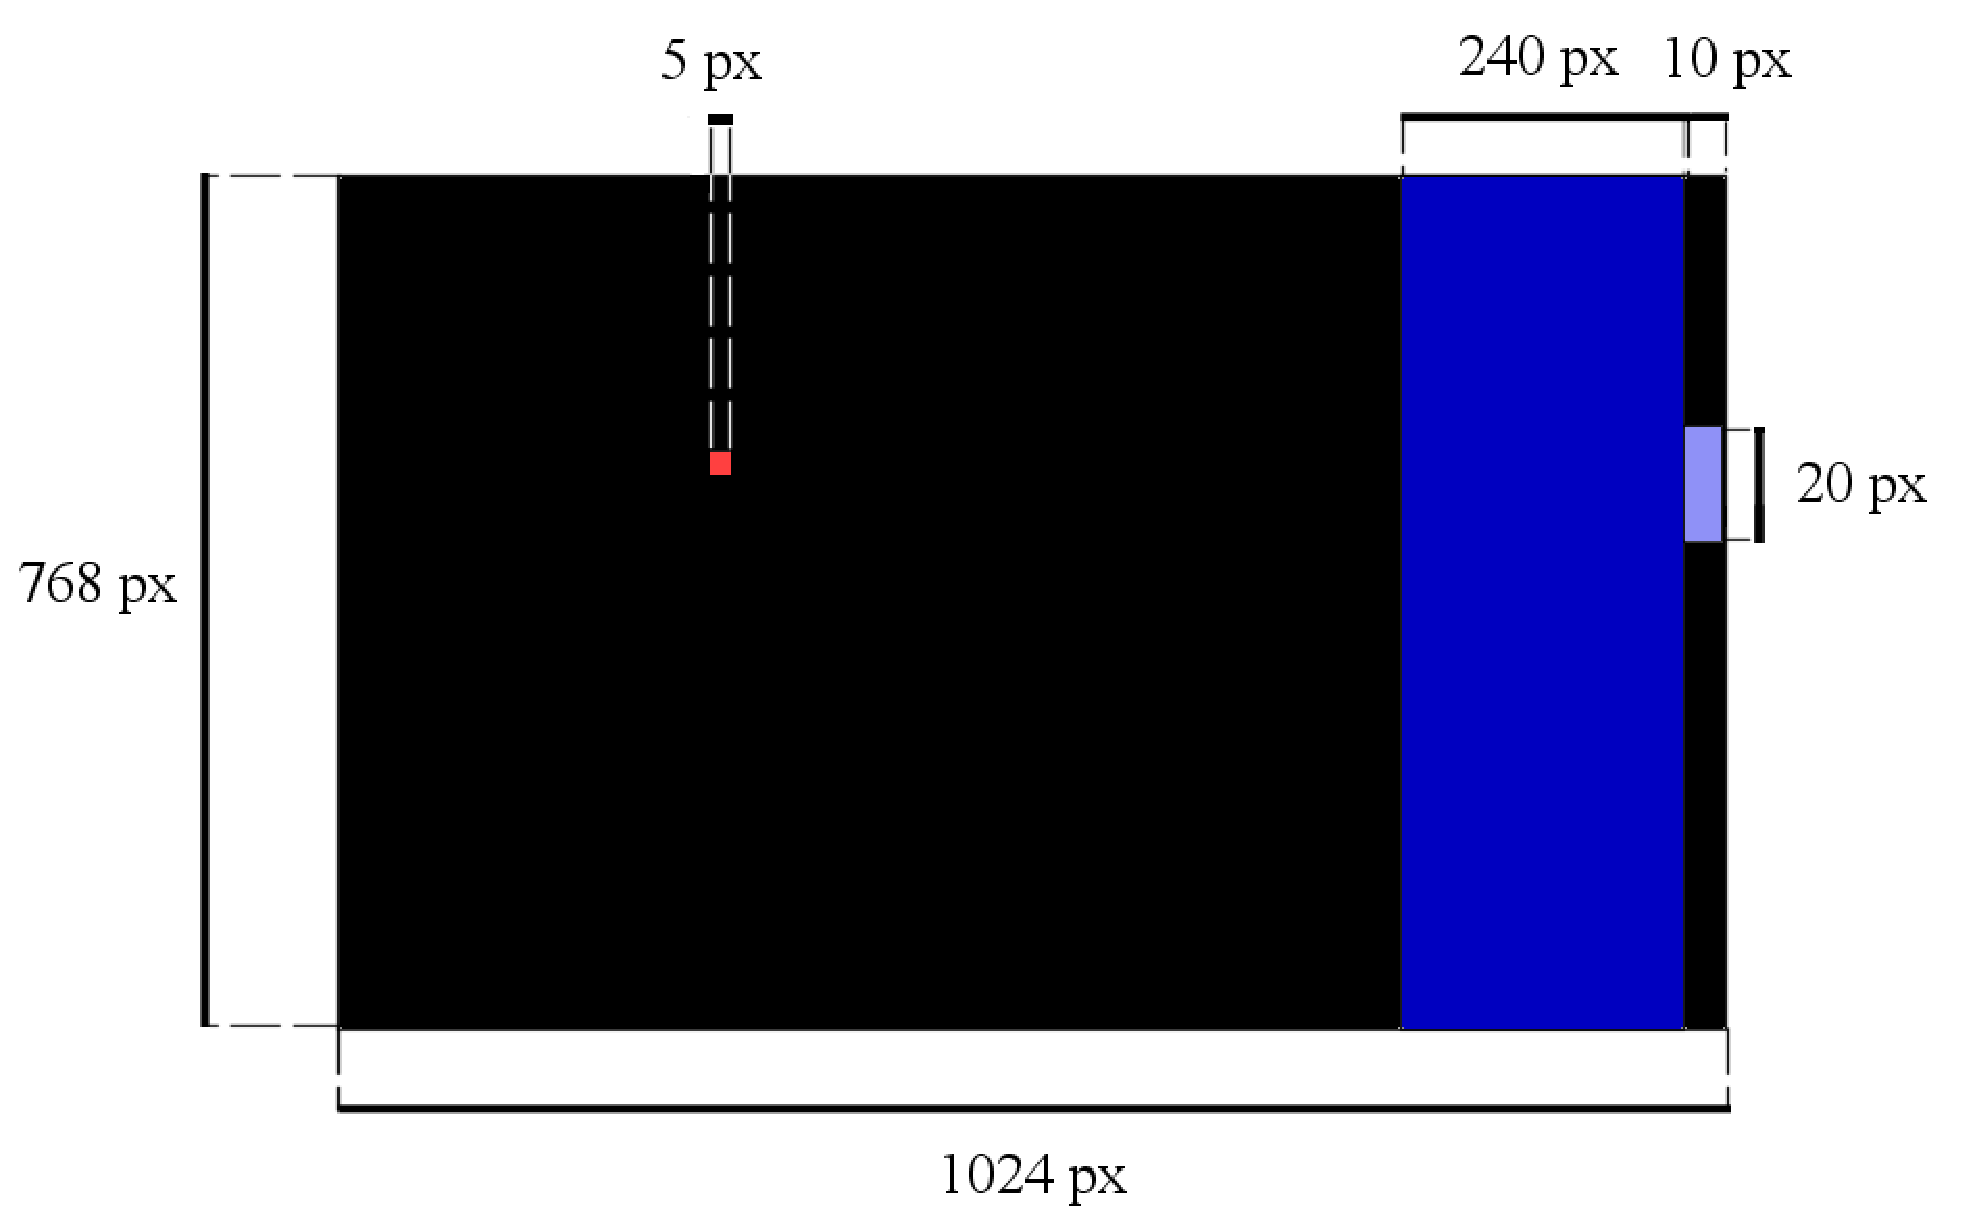
\includegraphics[width=15cm]{fig/schema_pong.eps}
	\caption{Video game screen sketch. A px (pixel) corresponds to 0.026 cm.}
	\label{figSchemaPong}
\end{figure}



%The wall width was designed together with the horizontal velocity component of the 
%ball in order to hide the ball at least for 200 ms. In this way even for the fastest trials subjects had the time 
%to execute an interception task, despite the visuo-motor delays typical of humans, estimated around 200 ms.

\subsection{Task}

Subjects were requested to intercept the ball with the paddle, as soon as it arrived at the extreme right of the screen.  They got one point if they intercepted the target with the center of the paddle, half a point if they touched it only with one side of the paddle and zero points in case of a miss. In addition at the end of each trial a yellow dot appeared for about 200 ms to show the position where the ball disappeared. They were encouraged to reach a score as high as possible. An ''error'' was also measured as the absolute difference between the vertical position of the ball center and that of the paddle center at the interception time. Subjects could see during the experiment how many trials they had already made, how much was their total score and their last error. They had also the possibility to stop and resume the game at any time, by pressing a key.


\subsection{Protocols}

The visual target appeared from the left side of the screen with pseudorandomly assorted initial vertical positions
($y_0 \in \left[0,\;20\right]\;cm $) and initial speeds ($v_0 \in \left[10\; cm/s, 10\; m/s \right]$) and crossed the screen with parabolic trajectories. The acceleration varied according to two different conditions (\textit{test} and \textit{control}), but in both cases was directed vertically, i.e. $a_x=0$. One experimental session consisted of 15 blocks of 65 trials each. At the end of each block the game paused and was up to the subject to decide when to resume it. The user could in this way rest the time subjectively needed. The average duration of a session was about an hour.

The two conditions differed in how the parabolic trajectories of the ball were generated\footnote{Remarkably, in all the experimental conditions, the same ball trajectory was never presented twice to the same subject. Therefore, catching performance could only be improved by understanding the way trajectories are generated.}. The \textit{control} group (9 subjects) had to intercept trajectories which were not produced by a unique underlying force field. Specifically, each trial presented a different acceleration $a_y$, both in modulus and direction [upward - downward]. In the \textit{test} group each trial (excluding the 14th block) was generated by the same dynamical system. In particular the ball moved in a constant vertical force field and was then affected by a constant acceleration (i.e. $a_y$ did not vary during the experiment)\footnote{Different parabolic trajectories were produced by changing only the initial conditions $y_0$ and $\underline{v}_0$.}. The 14th block of trials in the \textit{test} condition had the same features of a \textit{control} condition, i.e. the acceleration was changed at the beginning of each trial. Furthermore, the group of \textit{test} subjects was divided into two subgroups, according to the direction of the acceleration: downward $a_y=-0.325 m/{s^2}$ (10 subjects) versus upward $a_y=+0.325 m/{s^2}$ (9 subjects) orientation.

\textcolor{red}{The initial values of $y_0$ and $\underline{v}_0$ used to characterize the different trajectories were chosen in order to assure that each condition was different from the others only because of the different force field (i.e. acceleration): the time of flight of the ball % (see Fig.\ref{figTempi})
and the distribution of the arrival points of the trajectories are comparable for the three groups. Furthermore also the variance of the arrival point for each block of 65 trials is kept constant (see Fig.\ref{figCondInit}). % (see Fig.\ref{figStdOrdinate}). 
In this way these parameters could not determine differences in performance among conditions. In addition trajectories which ended in peripheral points of the screen were avoided and only those which arrived in the central 500 pixel were accepted.}



\begin{figure}[tbp]
	\centering
		\includegraphics[width=15cm]{fig/figOrdinate.eps}
		\includegraphics[width=15cm]{fig/figHistOrdinate.eps}
		\includegraphics[width=8cm]{fig/figTempi.eps}
		\includegraphics[width=8cm]{fig/figStdOrdinate.eps}
	\caption{\textbf{Above} - Ball arrival points in the three experimental conditions. \textbf{Center} -  Ball arrival points distribution in the three experimental conditions. \textbf{Below} - \textit{Left}: Flight time distribution in the three different conditions, \textit{Right}: block standard deviation of the ball arrival points in the three different conditions.}
	\label{figCondInit}
\end{figure}

%\begin{figure}[tbp]
%	\centering
%		\includegraphics[width=8cm]{fig/figTempi.eps}
%			\includegraphics[width=8cm]{fig/figStdOrdinate.eps}
%	\caption{Flight time distribution in the three different conditions and block standard deviation of the ball arrival points.}
%	\label{figTempi}
%\end{figure}

%% Alternativamente, figure separate.

%\begin{figure}[tbp]
%	\centering
%		\includegraphics[width=15cm]{fig/figTempi.eps}
%	\caption{Flight time distribution in the three different conditions . }
%	\label{figTempi}
%\end{figure}

%\begin{figure}[tbp]
%	\centering
%		\includegraphics[width=15cm]{fig/figStdOrdinate.eps}
%	\caption{Block standard deviation of the ball arrival points.}
%	\label{figStdOrdinate}
%\end{figure}

\subsection{Statistics}
Differences between each pair of conditions were assessed using single- or multiple- factor
ANOVA. The threshold for statistical significance was set at $\alpha =
0.05$. Statistically significant differences of mean errors among all the three
experimental conditions were assessed using multiple comparison procedures as Tukey's honestly significant difference criterion \citep{Hochberg}.